% Description of the paper meetings and their explanation

\section{Meetings}
Retaining the exact same number of players requires rounding up the number of players each strategy possesses and then redistributing the decimal parts, which ultimately add up to either one or two, to a specific strategy or a group of strategies. The method we figured produced the most accurate to the 1999's paper results was distributing the decimal parts to the strategy that was the closest to its next integer. It is important to note that changes in this procedure could lead to largely different results.

\subsection{Defectors may be strong}
\begin{figure}[H]
    \centering
    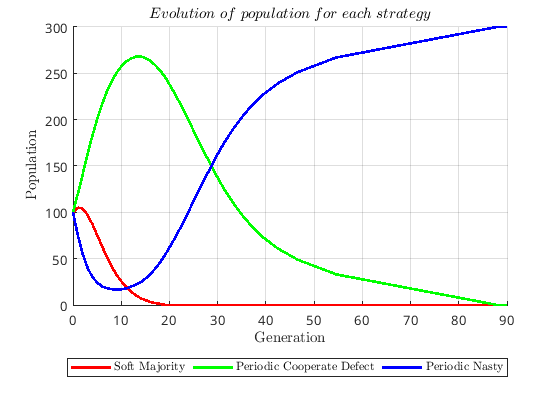
\includegraphics[width=0.8\textwidth]{media/meetings/defectors_may_be_strong.png}
    \caption{Defectors may be strong Plot}
\end{figure}

\subsection{Monotonous convergence}
\begin{figure}[H]
    \centering
    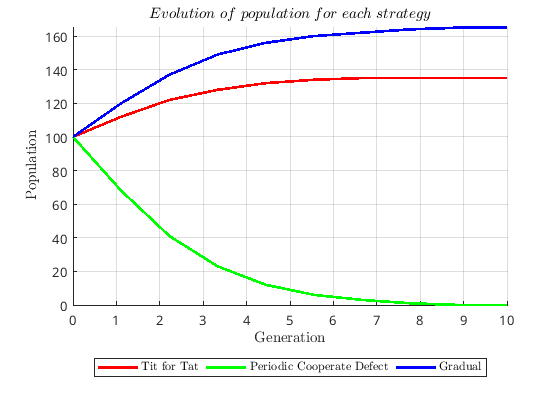
\includegraphics[width=0.8\textwidth]{media/meetings/monotonous_convergence.png}
    \caption{Monotonous convergence Plot}
\end{figure}

\subsection{Periodic movements}
\begin{figure}[H]
    \centering
    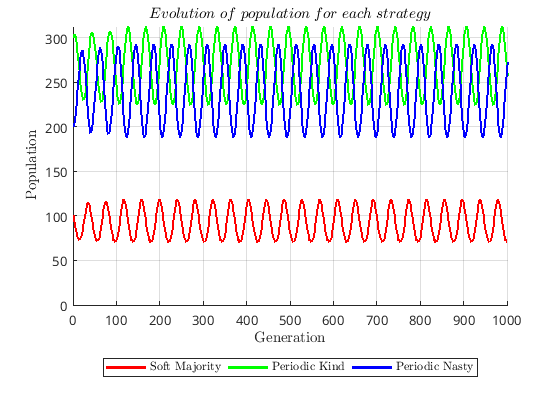
\includegraphics[width=0.8\textwidth]{media/meetings/periodic_movements.png}
    \caption{Periodic movements Plot}
\end{figure}

\subsection{Increasing oscillations}
\begin{figure}[H]
    \centering
    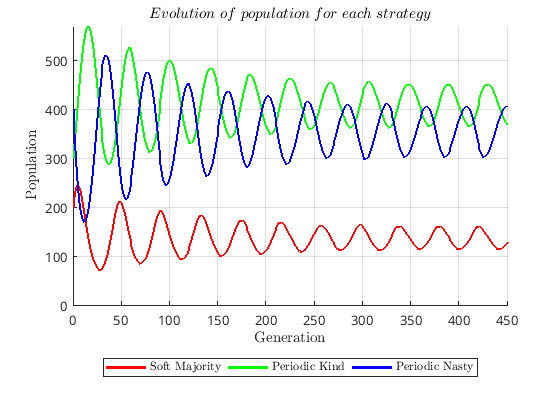
\includegraphics[width=0.8\textwidth]{media/meetings/increasing_oscillations.png}
    \caption{Increasing oscillations Plot}
\end{figure}

\subsection{Disordered oscillations}
\begin{figure}[H]
    \centering
    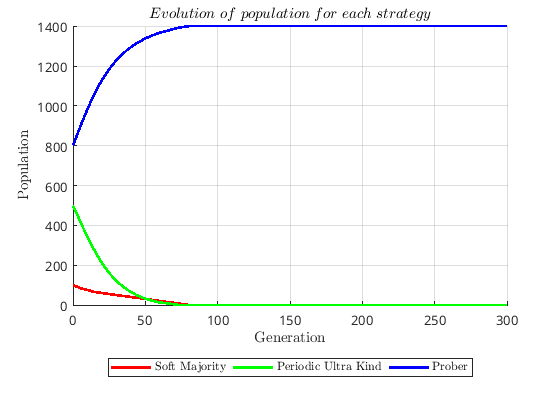
\includegraphics[width=0.8\textwidth]{media/meetings/disordered_oscillations.png}
    \caption{Disordered oscillations Plot}
\end{figure}
